Энэ хэсэгт Монгол Ай Ди компанийн хөгжүүлж буй MinuPOS системийн зээлийн хэсэгт харьяалагдах банкны Excel хуулгыг боловсруулах модуль болон түүнтэй холбогдох асуудлыг шийднэ.
\section{MinuPOS системийн банкны Excel хуулгыг боловсруулах модулийн шинжилгээ}
Тус модуль нь банкнаас ирсэн Excel файлыг автоматаар уншиж, өгөгдлийг шалган, шаард- лагатай тохиолдолд алдааг илрүүлж, мэдээллийг MinuPOS системийн өгөгдлийн санд шууд хадгалах боломжийг бүрдүүлнэ.
\subsection{MinuPOS системийн танилцуулга}
MinuPOS нь бизнес эрхлэгчид болон жижиг дунд аж ахуйн нэгжүүдийн санхүүгийн хэрэг- цээг хангах цогц зээлийн систем бүхий платформ юм. Эдгээр зээлийн үйлчилгээнүүдийг MinuPOS-ийн мобайл аппликейшн болон POS системээс шууд удирдах боломжтой бөгөөд ингэснээр зээлийн хүсэлт гаргах, төлбөрийн түүхээ харах, POS орлоготой уялдуулан зээлийн төлөлтөө автоматжуулах зэрэг үйлдлийг цахимаар хийх боломжтой. MinuPOS нь Монголын 12 банкны санхүүгийн системтэй шууд холбогдож, хэрэглэгчдийн банкны хуулгыг автоматаар татаж авч, тэдгээрийг боловсруулан зээлийн мэдээлэлтэй уялдуулдаг. Энэ нь хэрэглэгчдэд цаг хугацаа хэмнэх, гар ажиллагааг багасгах, мөн зээлийн эрсдэлийг бууруулахад тусалдаг. MinuPOS нь мөн QR кодын төлбөрийн системийг дэмждэг бөгөөд энэ нь хэрэглэгчдэд хурдан, аюулгүй төлбөр хийх боломжийг олгодог.

\subsection{Одоогийн MinuPOS системийн банкны Excel хуулгыг боловсруулах модульд тулгарч буй асуудал}
Монголын 12 банк тус бүр өөрийн гэсэн Excel хуулгын форматыг ашигладаг тул эдгээр форматуудыг зөв таньж, боловсруулах нь төвөгтэй байдаг. Иймд одоогийн  MinuPOS системийн банкны Excel хуулгыг боловсруулах модульд формат бүрт зориулсан урт хэмжээтэй өөр өөр код бичигдсэн байгааг сайжруулах хэрэгтэй байна. Мөн зарим банкны Excel хуулгын форматууд нь цаг хугацааны явцад өөрчлөгдөж, шинэчлэгддэг тул эдгээр өөрчлөлтүүдийг код дээр гар аргаар засварлах шаардлагатай болж, энэ нь алдаа гарах магадлалыг нэмэгдүүлдэг. Түүнчлэн зарим тохиолдолд хэрэглэгчид буруу форматтай эсвэл шаардлага хангахгүй Excel файлуудыг оруулдаг тул эдгээр алдааг илрүүлж, хэрэглэгчдэд ойлгомжтой мэдээлэл өгөх механизм дутагдалтай байна.

\subsection{Системийн орчин}

MinuPOS системийн системийн сервер талын код нь Жава технологи дээр бичигдсэн ба үндсэн фреймворк нь Spring Boot юм. MinuPOS нь SoftPOS шийдэлтэй; ухаалаг утсаар карт/NFC төлбөр хүлээн авах боломжийг MineSec SoftPOS\footnote{https://minesecsoftpos.com/}-оор хангадаг.
MinuPOS системийн худалдан авагч/борлуулагч талын интерфэйс нь POS терминал, SoftPOS, нэгдсэн QR дээр суурилна. Борлуулагч талын Монгол Ай Ди компанийн хөгжүүлсэн iOS/Android мобайл аппууд нийтэд байршсан.
MinuPOS систем нь PostgreSQL харьцаат өгөгдлийн санг ашигладаг. 
\newpage
\subsection{Динамик загвар}
MinuPOS системийн банкны Excel хуулгыг боловсруулах модулийн ажлын явцын диаграмыг \ref{fig:module_usecase} зурагт үзүүлэв. 

% @startuml
% left to right direction
% skinparam packageStyle rectangle

% actor Хэрэглэгч as U
% actor Админ as A

% rectangle "\tMinuPOS системийн банкны Excel хуулгыг боловсруулах модуль\t" {
%   usecase "Банкны хуулга оруулах" as UC1
%   usecase "Банкны загвар сонгох" as UC2
%   usecase "Багануудыг буулгах" as UC3
%   usecase "Өгөгдлийг баталгаажуулах" as UC4
%   usecase "Гүйлгээнүүдийг хадгалах" as UC5
%   usecase "Гүйлгээнүүд дээр\n асуулга хийх" as UC6
%   usecase "Банкны загваруудыг \n зохион байгуулах" as UC7
  
%   U --> UC1 : <<include>>
%   U --> UC2 : <<include>>
%   U --> UC3 : <<extend>>\n Хэрэв шинэ загвар\n үүссэн бол
%   U --> UC4
%   U --> UC6
%   A --> UC7 : <<extend>>
  
%   UC1 .> UC2 : <<include>>
%   UC2 .> UC3 : <<extend>>
%   UC3 .> UC4 : <<include>>
%   UC4 .> UC5 : <<include>>
% }
% @enduml

\begin{figure}[h]
		\centering
		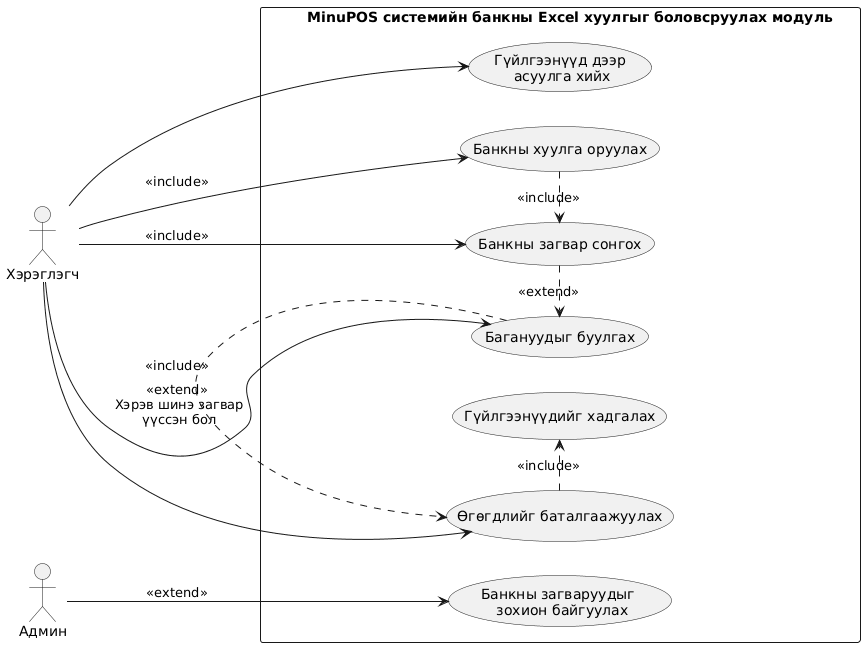
\includegraphics[width=17cm]{images/module_usecase.png}
		\caption{MinuPOS системийн банкны Excel хуулгыг боловсруулах модулийн ажлын явцын диаграм}
		\label{fig:module_usecase}
\end{figure}

Дээрх ажлын явцын диаграмд тусгасан чухал ажлын явцын тайлбаруудыг харгалзах \ref{tab:ucfs01} болон \ref{tab:ucfs02} хүснэгтүүдэд үзүүлэв. Энд ажлын явцын өдөөгч үзэгдэл, тоглогч, угтвар нөхцөл, дараах нөхцөл, үр дүн, тайлбар, өргөтгөл, хувилар болон чанарын шаардлагуудыг тус тус харгалзан үзэв.

%------------------------------------------------------------------------
\begin{longtable}{|L{4cm}|L{\dimexpr\textwidth-4cm-3\tabcolsep-2\arrayrulewidth\relax}|}
\caption{Ажлын явц: Банкны хуулга оруулах (UC-FS-01)}\label{tab:ucfs01}\\ \hline
\textbf{Хэсэг} & \textbf{Агуулга} \\ \hline
\endfirsthead

\multicolumn{2}{c}{\tablename\ \thetable\ -- \textit{үргэлжлэл}} \\ \hline
\textbf{Хэсэг} & \textbf{Агуулга} \\ \hline
\endhead

\hline \multicolumn{2}{r}{\textit{(үргэлжилнэ)}} \\ \hline
\endfoot

\hline
\endlastfoot

Тэмдэглэгээ & UC-FS-01 \\ \hline
Ажлын явцын нэр & Банкны хуулга оруулах \\ \hline
Ангилал & Анхдагч \\ \hline
Тодорхойлолт & Хэрэглэгч нь Монголын 12 банкны аль нэгээс Excel хуулга оруулж, стандарт хэлбэрт шилжүүлэн хадгалах боломжтой. \\ \hline
Өдөөгч үзэгдэл & Хэрэглэгч веб интерфейсээр файл оруулахыг эхлүүлсэн үед \\ \hline
Тоглогч & Банкны хэрэглэгч, Template Mapping үйлчилгээ, Data Validator, PostgreSQL өгөгдлийн сан \\ \hline
Угтвар нөхцөл & 1. Банкны загвар байгаа эсвэл үүсгэж болно.\\ \hline
Дараах нөхцөл & 1. Гүйлгээний мэдээлэл өгөгдлийн санд хадгалагдсан байна.\\
                & 2. Хэрэглэгч үр дүнгийн мэдээлэл авсан байна. \\ \hline
Үр дүн & Стандартчлагдсан санхүүгийн мэдээлэл хэрэглэгчийн атрибутаар хадгалагдсан байна. \\ \hline
Тайлбар & 1. Модуль нь Excel файл болон хэрэглэгчийн сонгосон метадатаг хүлээн авна.\\
              & 2. Метадатагаас банкны төрлийг тодорхойлно.\\
              & 3. Баганын буулгалтын загварыг авна.\\
              & 4. Тохиргооны дүрмээр гүйлгээг задлана.\\
              & 5. Өгөгдлийн бүрэн бүтэн байдал шалгагдана.\\
              & 6. Стандарт $\digamma$ хэлбэрт хөрвүүлнэ.\\
              & 7. Өгөгдлийн санд хадгална.\\ \hline
Өргөтгөл & 3a. Загвар байхгүй тохиолдолд: \\ 
                      & \quad 3a1. Модуль нь баганын буулгалтын загварыг асууна. \\ 
                      & \quad 3a2. Хэрэглэгч талбаруудыг тодорхойлно. \\ 
                      & \quad 3a3. Шинэ загвар үүснэ. \\ 
                      & 5a. Буруу өгөгдөл илэрсэн тохиолдолд: \\ 
                      & \quad 5a1. Хэрэглэгч засаж дахин оруулна. \\ \hline
Онцгой тохиолдол & Өдөөгч: Танигдаагүй файл формат.\\ 
                    & Өдөөгч: Өгөгдлийн сангийн холболт тасарсан.\\ 
                    & Өдөөгч: Засаж болохгүй буруу өгөгдөл. \\ \hline
Чанарын шаардлага & QR-01 (Өгөгдлийн үнэн зөв байдал: 99.9\%)\\ 
          & QR-12 (GDPR нийцтэй байдал)\\ 
          & QR-07 (10,000 бичлэгийг $<$20 секундэд боловсруулна) \\ \hline

\end{longtable}
%------------------------------------------------------------------------
\begin{longtable}{|L{4cm}|L{\dimexpr\textwidth-4cm-3\tabcolsep-2\arrayrulewidth\relax}|}
\caption{Ажлын явц: Банкны загвар үүсгэх (UC-FS-02)}\label{tab:ucfs02}\\ \hline
\textbf{Хэсэг} & \textbf{Агуулга} \\ \hline
\endfirsthead

\multicolumn{2}{c}{\tablename\ \thetable\ -- \textit{үргэлжлэл}} \\ \hline
\textbf{Хэсэг} & \textbf{Агуулга} \\ \hline
\endhead

\hline \multicolumn{2}{r}{\textit{(үргэлжилнэ)}} \\ \hline
\endfoot

\hline
\endlastfoot

Тэмдэглэгээ & UC-FS-02 \\ \hline
Ажлын явцын нэр & Банкны загвар үүсгэх \\ \hline
Ангилал & Анхдагч \\ \hline
Тодорхойлолт & Админ нь шинэ банкны хуулгын форматын баганануудын буулгалтыг тодорхойлж, загвар үүсгэнэ. \\ \hline
Өдөөгч үзэгдэл & Шинэ банк нэмэгдсэн эсвэл форматыг өөрчилсөн тохиолдолд \\ \hline
Тоглогч & Админ \\ \hline
Угтвар нөхцөл & 1. Жишиг хуулга бэлэн байна.\\
               & 2. Стандарт талбарууд тодорхойлогдсон байна. \\ \hline
Дараах нөхцөл & 1. Шинэ загвар хувилбар хадгалагдсан байна.\\ \hline
Үр дүн & Банкны хуулгад ашиглах дахин ашиглах боломжтой буулгалт бүхий загвар үүссэн байна. \\ \hline
Тайлбар & 1. Админ жишиг хуулгыг оруулна.\\
              & 2. Админ багануудыг стандарт талбаруудад буулгана.\\
              & 3. Модуль нь буулгалтын бүрэн бүтэн байдлыг шалгана.\\
              & 4. Загвар хадгалагдана.\\ \hline
Өргөтгөл & 4a. Буулгалт гүйцээгүй тохиолдолд: \\
                      & \quad 4a1. Модуль нь дутагдсан талбаруудыг онцолж харуулна. \\
                      & \quad 4a2. Админ нэмэлт буулгалт оруулна. \\[4pt]
                      & 5a. Өмнөх загвартой зөрчилдөөн гарвал: \\
                      & \quad 5a1. Хувилбаруудын харьцуулалтыг харуулна. \\
                      & \quad 5a2. Админ давхарлах эсэхийг баталгаажуулна. \\ \hline
Онцгой тохиолдол & Өдөөгч: Буруу буулгалтын загвар.\\
                    & Өдөөгч: Хадгалах квота хэтэрсэн. \\ \hline
Чанарын шаардлага & QR-09 (загвар үүсгэх хугацаа $<$ 5 минут)\\
          & QR-14 (Хувилбар зөрчилөөс урьдчилан сэргийлэх)\\ \hline

\end{longtable}


\newpage
\subsection{Функциональ  шаардлага}
Доор MinuPOS системийн банкны Excel хуулгыг боловсруулах модулийн функциональ шаардлагуудыг жагсаав. Дадлага удирдагчийн заавраар хэрэглэгч нэвтрэх/бүртгэх шаардлагыг орхигдуулсан болно. Хэрэглэгч нь админ байж болно.
\begin{table}[h]
\caption{Банкны Excel хуулгыг боловсруулах модулийн функциональ шаардлага}
\begin{tabular}{|p{3cm}|p{13cm}|}
\hline
Шаардлагын нэр & \text{Шаардлагын тайлбар} \\ \hline
ФШ10 & Модуль нь банкны Excel хуулгаас гүйлгээний мэдээллийг (огноо, дүн, тайлбар) уншиж авна. \\ \hline
ФШ11 & Модуль нь өгөгдсөн банкны Excel хуулгаас уншиж авсан мэдээллийг  $\digamma$ стандарт бүтэцтэй объектод хувиргана. $\digamma$ стандарт бүтцийн дэлгэрэнгүйг "Өгөгдлийн бүтэц ба загвар" хэсгээс харна уу. \\ \hline
ФШ12 & Модуль нь өгөгдсөн банкны Excel хуулгын мэдээллийг өгөгдлийн санд хадгалдаг байна. \\ \hline
ФШ13 & Модуль нь хадгалсан гүйлгээнүүд дээр огноо, дүн, тайлбар зэрэг атрибутуудаар хайлт хийх боломжийг олгодог байна. \\ \hline
ФШ20 & Модуль нь хэрэглэгчээс банкны төрлийг оролтоор авдаг байна. \\ \hline
ФШ21 & Модуль нь хэрэглэгчид банкны Excel хуулгын загварыг оролтоор оруулах боломжийг олгодог байна. \\ \hline
ФШ30 & Модуль нь хэрэглэгчээс банкны Excel хуулгыг оролтоор авдаг байна. \\ \hline
ФШ40 & Модуль нь хэрэглэгчид банкны загвар үүсгэх боломжийг олгодог байна. \\ \hline
ФШ41 & Модуль нь хэрэглэгчид хадгалсан банкны загваруудыг засах, устгах боломжийг олгодог байна. \\ \hline
\end{tabular}
\end{table}

\newpage
\subsection{Функциональ бус шаардлага}
\begin{table}[h]
\caption{Банкны Excel хуулгыг боловсруулах модулийн функциональ бус шаардлага}
\begin{tabular}{|p{3cm}|p{13cm}|}
\hline
Шаардлагын нэр & \text{Шаардлагын тайлбар} \\ \hline
ФШБ10 & 1000 хүртэлх мөр бүхий Excel хуулгыг 5 секундын дотор боловсруулж, өгөгдлийн санд амжилттай хадгалдаг байна. \\ \hline
ФБШ20 & Хэрэглэгчийн Excel хуулга оруулах үйлдэл нь ойлгомжтой, 3-аас илүүгүй алхмаар хийгддэг байна. \\ \hline
ФБШ40 & Модуль нь шинэ банкны төрөл эсвэл загварыг нэмэхэд хялбар, үүнийг хийхэд одоо байгаа кодонд их хэмжээний өөрчлөлт хийх шаардлагагүй байна. \\ \hline
ФБШ41 & Код нь цэгцтэй, тайлбар бичигдсэн, өөр хөгжүүлэгч тухайн кодыг ойлгоход хялбар байна. \\ \hline
\end{tabular}
\end{table}

\subsection{Хөгжүүлэлтийн орчинд тавигдах шаардлага}

\begin{table}[h]
\caption{Банкны Excel хуулгыг боловсруулах модулийн хөгжүүлэлтийн орчинд тавигдах шаардлага}
\begin{tabular}{|p{3cm}|p{13cm}|}
\hline
Шаардлагын нэр & \text{Шаардлагын тайлбар} \\ \hline
ХОТШ10 & Модуль хөгжүүлэхэд зориулсан нэгдсэн
хөгжүүлэлтийн орчинг (IDE) ашиглана. \\ \hline
ХОТШ20 & Git зэрэг хувилбарын хяналтын системүүдийг ашигладаг байна. \\ \hline
ХОТШ30 & Өгөгдлийн хадгалахдаа PostgreSQL харьцаат өгөгдлийн санг ашиглана. \\ \hline
\end{tabular}
\end{table}

\newpage
\subsection{Өгөгдлийн бүтэц ба загвар}
Банкны Excel хуулгыг боловсруулах модуль нь $\digamma$ стандарт бүтэцтэй өгөгдлийн загварыг ашиглана. $\digamma$ стандарт бүтэц нь дараах төрөл бүхий талбарыг агуулна:
\subsubsection{Банкны хуулгын өгөгдлийн баганууд}
\begin{table}[h]
\centering
\caption{MinuPOS системийн $\digamma$ стандарт бүтцийн толгой баганууд}
\begin{tabular}{|p{5cm}|p{5cm}|}
\hline
\textbf{Баганы нэр} & \textbf{Өгөгдлийн төрөл} \\ \hline
STATEMENT\_ID & VARCHAR2(20) \\ \hline
REQUEST\_ID & VARCHAR2(20) \\ \hline
BANK\_CODE & VARCHAR2(20) \\ \hline
START\_DATE & DATE \\ \hline
END\_DATE & DATE \\ \hline
TXN\_COUNT & NUMBER \\ \hline
INCOME & NUMBER \\ \hline
OUTCOME & NUMBER \\ \hline
FILE\_ID & VARCHAR2(100) \\ \hline
ACCOUNT\_NO & VARCHAR2(20) \\ \hline
CREATED\_DATE & DATE \\ \hline
STATEMENT\_DATE & DATE \\ \hline
MAIN\_FLAG & VARCHAR2(2) \\ \hline
ACCOUNT\_NAME & VARCHAR2(200) \\ \hline
\end{tabular}
\end{table}
\newpage
\subsubsection{Банкны хуулгын гүйлгээний дэлгэрэнгүй баганууд}
\begin{table}[h]
\centering
\caption{MinuPOS системийн $\digamma$ стандарт бүтцийн дэлгэрэнгүй баганууд}
\begin{tabular}{|p{5cm}|p{5cm}|}
\hline
\textbf{Баганы нэр} & \textbf{Өгөгдлийн төрөл} \\ \hline
DETAIL\_ID & VARCHAR2(20) \\ \hline
STATEMENT\_ID & VARCHAR2(20) \\ \hline
TXN\_DATE & DATE \\ \hline
PRE\_BALANCE & NUMBER \\ \hline
POST\_BALANCE & NUMBER \\ \hline
TXN\_AMOUNT & NUMBER \\ \hline
TXN\_TYPE & VARCHAR2(20) \\ \hline
TXN\_DESC & VARCHAR2(1000) \\ \hline
CO\_ACCOUNT & VARCHAR2(200) \\ \hline
USE\_FLAG & VARCHAR2(2) \\ \hline
USE\_FLAG\_USER\_ID & VARCHAR2(20) \\ \hline
USE\_FLAG\_DATE & DATE \\ \hline
STATUS & VARCHAR2(20) \\ \hline
\end{tabular}
\end{table}

Дадлагын ажлын хүрээнд миний гүйцэтгэх даалгавар нь асуудал шийдэх байсан тул шин- жилгээний үеийн классын диаграмыг үүсгээгүй болно. Гэхдээ статик загварыг доорх зохиом- жийн хэсэгт дэлгэрэнгүй тайлбарлав.

\newpage
\section{MinuPOS системийн банкны Excel хуулгыг боловсруулах модулийн зохиомж}
Энэ хэсэгт MinuPOS системийн банкны Excel хуулгыг боловсруулах модульд ашигласан гол архитектурын үлгэр загваруудыг танилцуулж, тэдгээрийн хэрэглээ, зохиомжийн тайлбарыг өгнө.

\subsection{"Strategy" үлгэр загварын зохиомжийн тайлбар}
Монголын банкууд Excel хуулгаа өөр өөр форматтайгаар өгдөг тул формат бүрт тусдаа, хатуу кодчилсон парсер бичих нь үр ашиггүй. "Strategy" үлгэр загварыг сонгосон гол шалтгаан нь шинэ банк нэмэх, эсвэл хуучин банкны хуулгын формат өөрчлөгдөхөд үндсэн парсингийн логикт өөрчлөлт хийх шаардлагагүй болоход оршино. Зөвхөн шинэ буулгалтын загвар нэмэхэд хангалттай. Ингэснээр код давхардал багасгаж чадна.
% Strategy Pattern-ийг хэрэг- жүүлснээр тухайн банкны Excel хуулгын буулгалтын тохиргоог (JSON хэлбэрээр хадгалсан) ачааллаж, runtime үед сонгосон банкны тохиргоонд тулгуурлан Excel файлыг боловсруулдаг болсон.

\subsection{"Template Method" үлгэр загварын зохиомжийн тайлбар}
Excel хуулга боловсруулахад "Template Method" үлгэр загварыг ашигласан. Ямар ч банкны Excel файлын хувьд ерөнхий алгоритм дараах алхмуудтай ижил байна:

\begin{figure}[h]
		\centering
		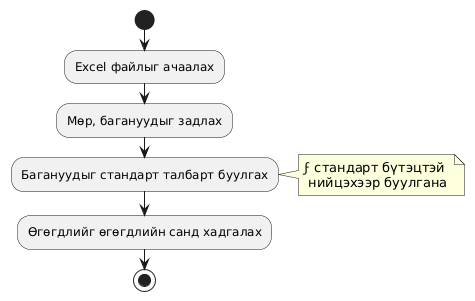
\includegraphics[width=10cm]{images/state.png}
		\caption{Excel хуулга боловсруулах ерөнхий төлөвийн диаграм}
		\label{fig:state}
\end{figure}

Энэ урсгал тогтмол боловч зарим алхам (жишээлбэл, багануудыг хэрхэн буулгах) нь банк бүрийн форматаас хамааран өөрчлөгдөж болно. Үүний тулд бүх хувилбар тус бүрээр дахин код бичихийн оронд ерөнхий алгоритмыг нэг загварт хадгалж, хувьсах алхмуудыг буулгалтын загвараар уян хатан болгож чадна. 

\subsection{"Factory" үлгэр загварын зохиомжийн тайлбар}

"Factory" үлгэр загварыг MappingConfigLoader классад тусгасан. Энэ класс нь буулгалтын загвар зэрэг объектуудыг үүсгэх үүрэгтэй бөгөөд тухайн объектыг хэрхэн бүтээх нарийн логикийг системийн бусад хэсэгт ил гаргахгүй. Жишээлбэл, JSON буулгалтын загварыг уншиж, тохирох буулгалтын объект үүсгэх ажлыг хариуцна.

\subsection{"Builder" үлгэр загварын зохиомжийн тайлбар}

Модуль тодорх StatementHdr, StatementDetail зэрэг энтити объектуудыг үүсгэхэд "Builder" үлгэр загварыг ашигласан (\ref{fig:builder} зургийг харна уу). Эдгээр энтитинүүд нь олон талбартай бөгөөд бүх утгууд нь нэг дор бэлэн байдаггүй. Барилгачин нь урт байгуулагч бичихгүйгээр, эсвэл бүх талбарыг гараар тохируулахгүйгээр объектуудыг алхам алхмаар үүсгэх боломжтой болгодог. Ирээдүйд шинэ талбар нэмэх шаардлага гарвал байгуулагч бүрийг өөрчлөхгүй, зөвхөн барилгачинд нэмэхэд хангалттай. (\ref{fig:builder} зургийг харна уу)
\begin{figure}[h]
		\centering
		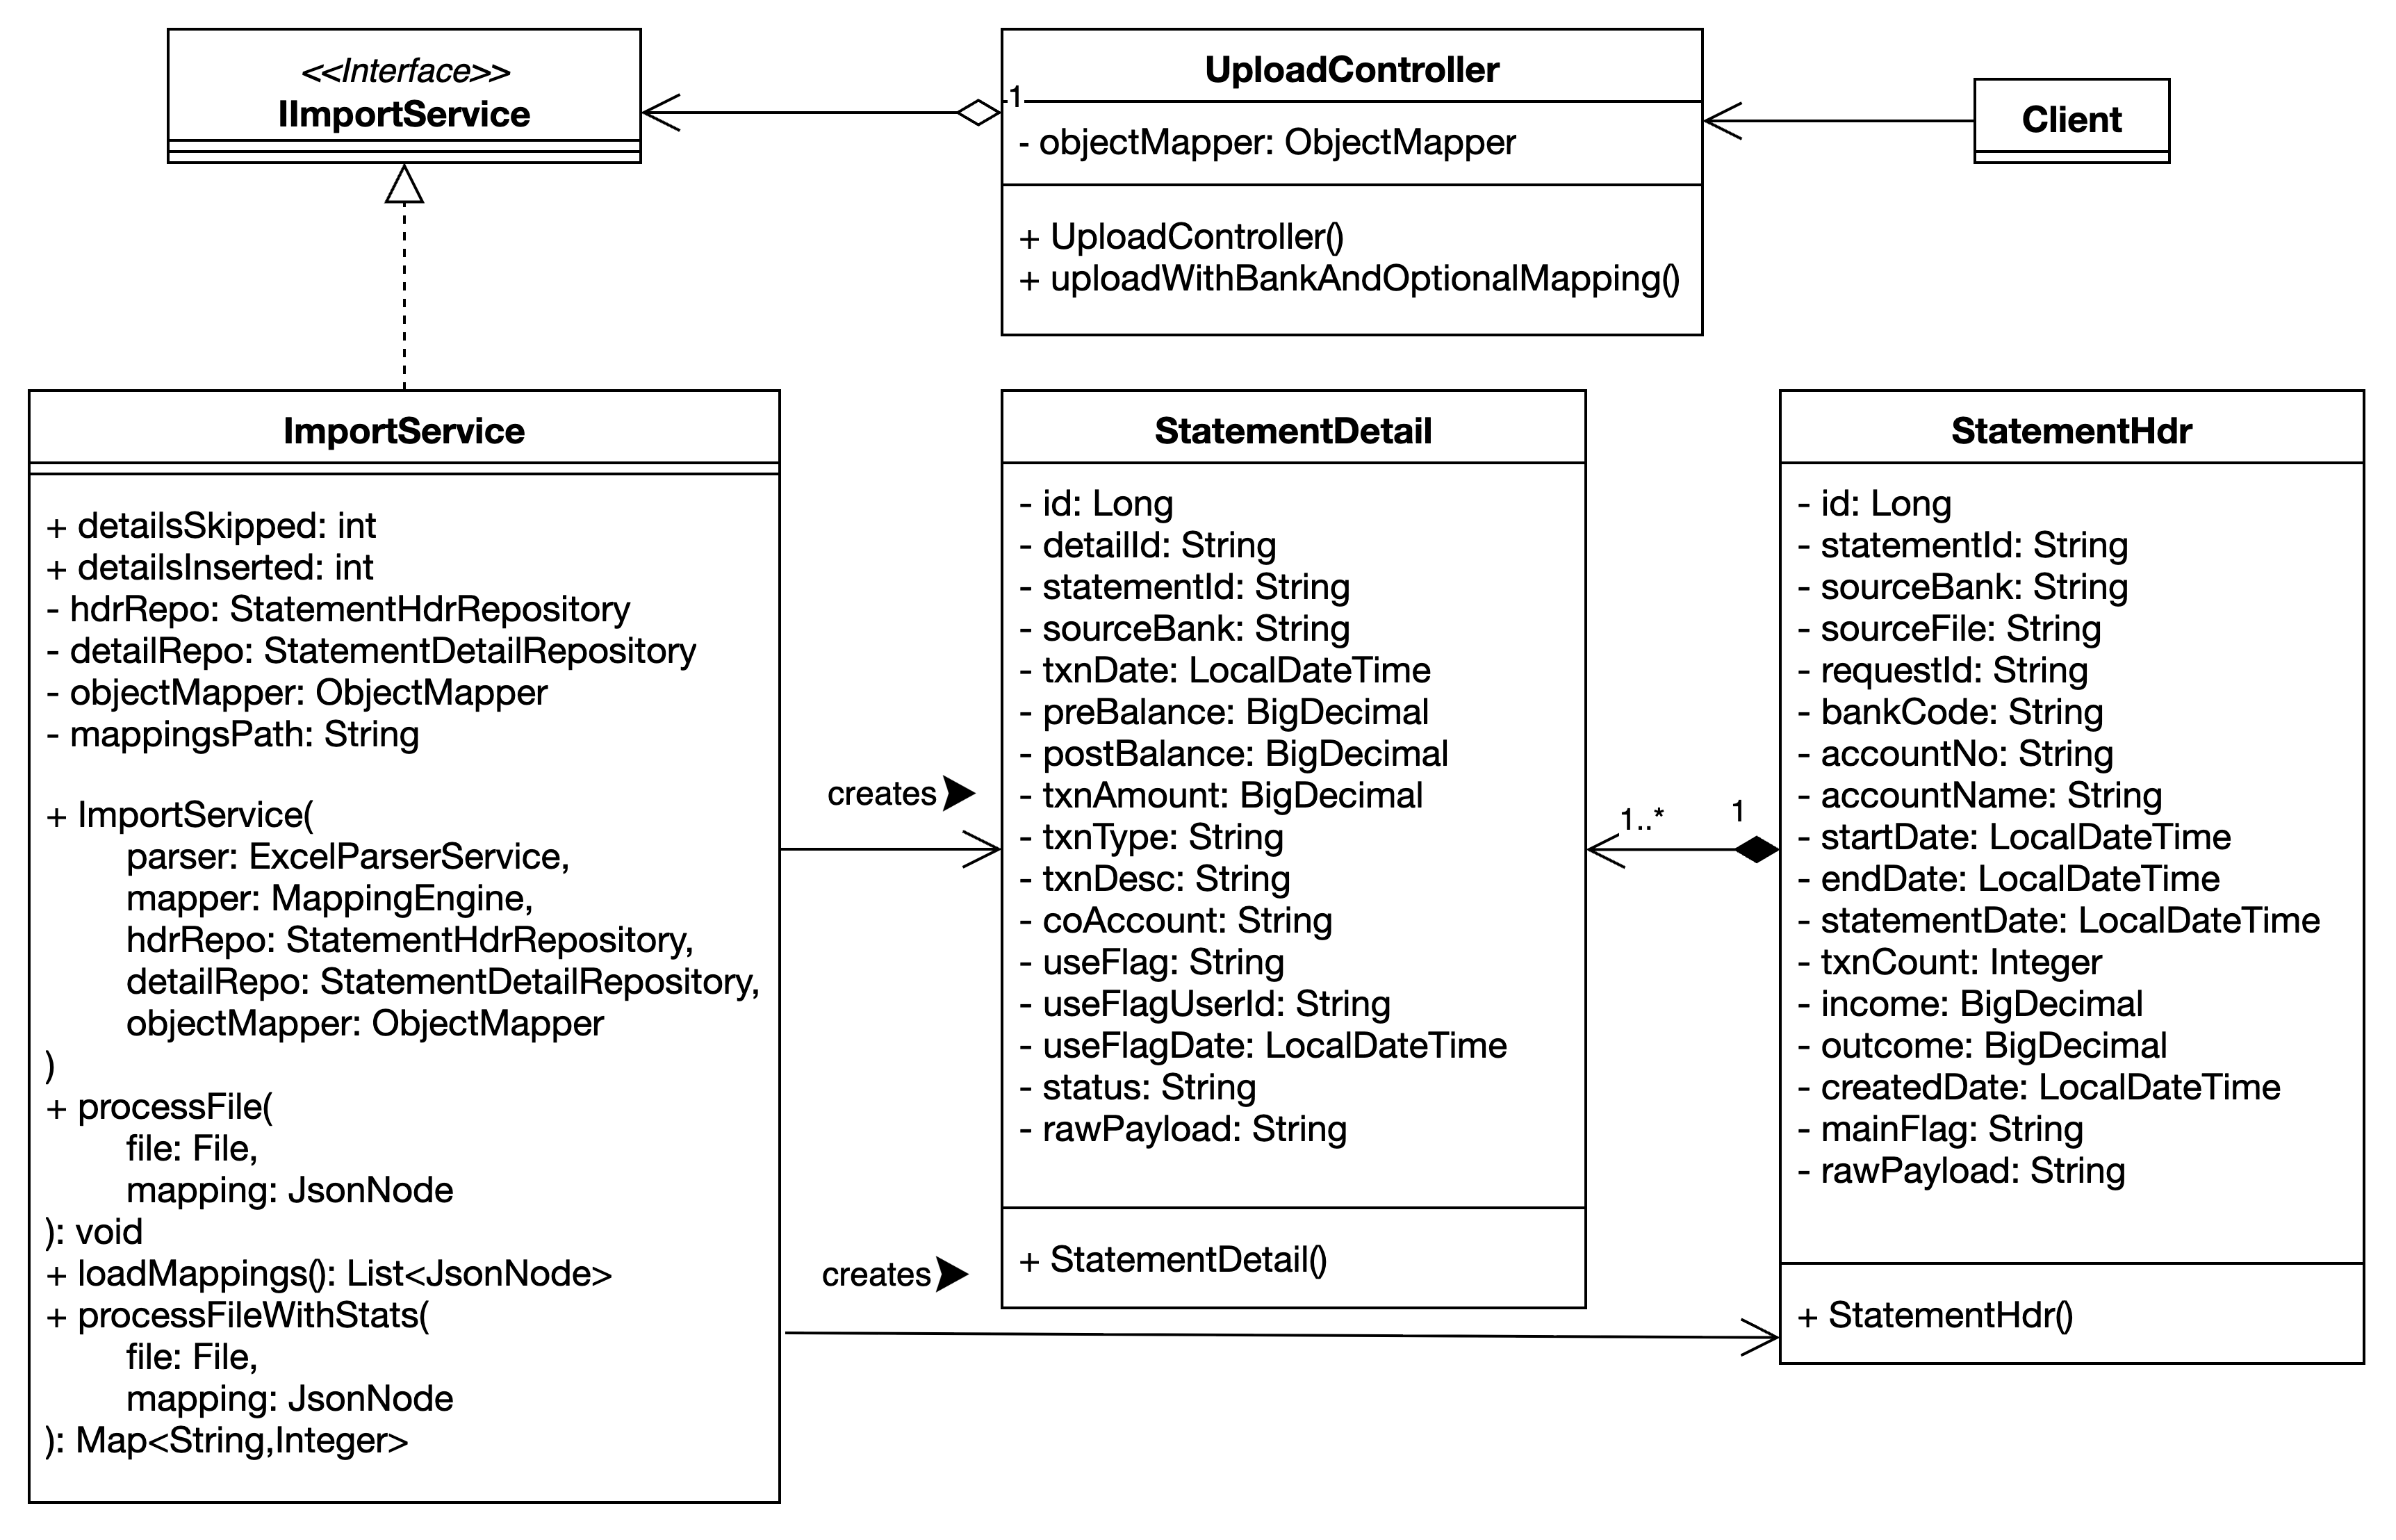
\includegraphics[width=15cm]{images/builder.png}
		\caption{"Builder" үлгэр загварын зохиомжийн диаграм}
		\label{fig:builder}
\end{figure}
\subsection{Модулийн статик загвар}
Шинжилгээний үед тодорхойлсон өгөгдлийн  $\digamma$ стандарт бүтэцтэй нийцэхээр model багцын классын диаграмыг \ref{fig:model} зурагт үзүүлэв. Мэдээж getter, setter, toString зэрэг агуудыг агуулах бөгөөд эдгээрийг диаграмд оруулаагүй болно. Модулийн гол зохиомжийн диаграмыг \ref{fig:design} зурагт үзүүлэв.

\begin{figure}[H]
		\centering
		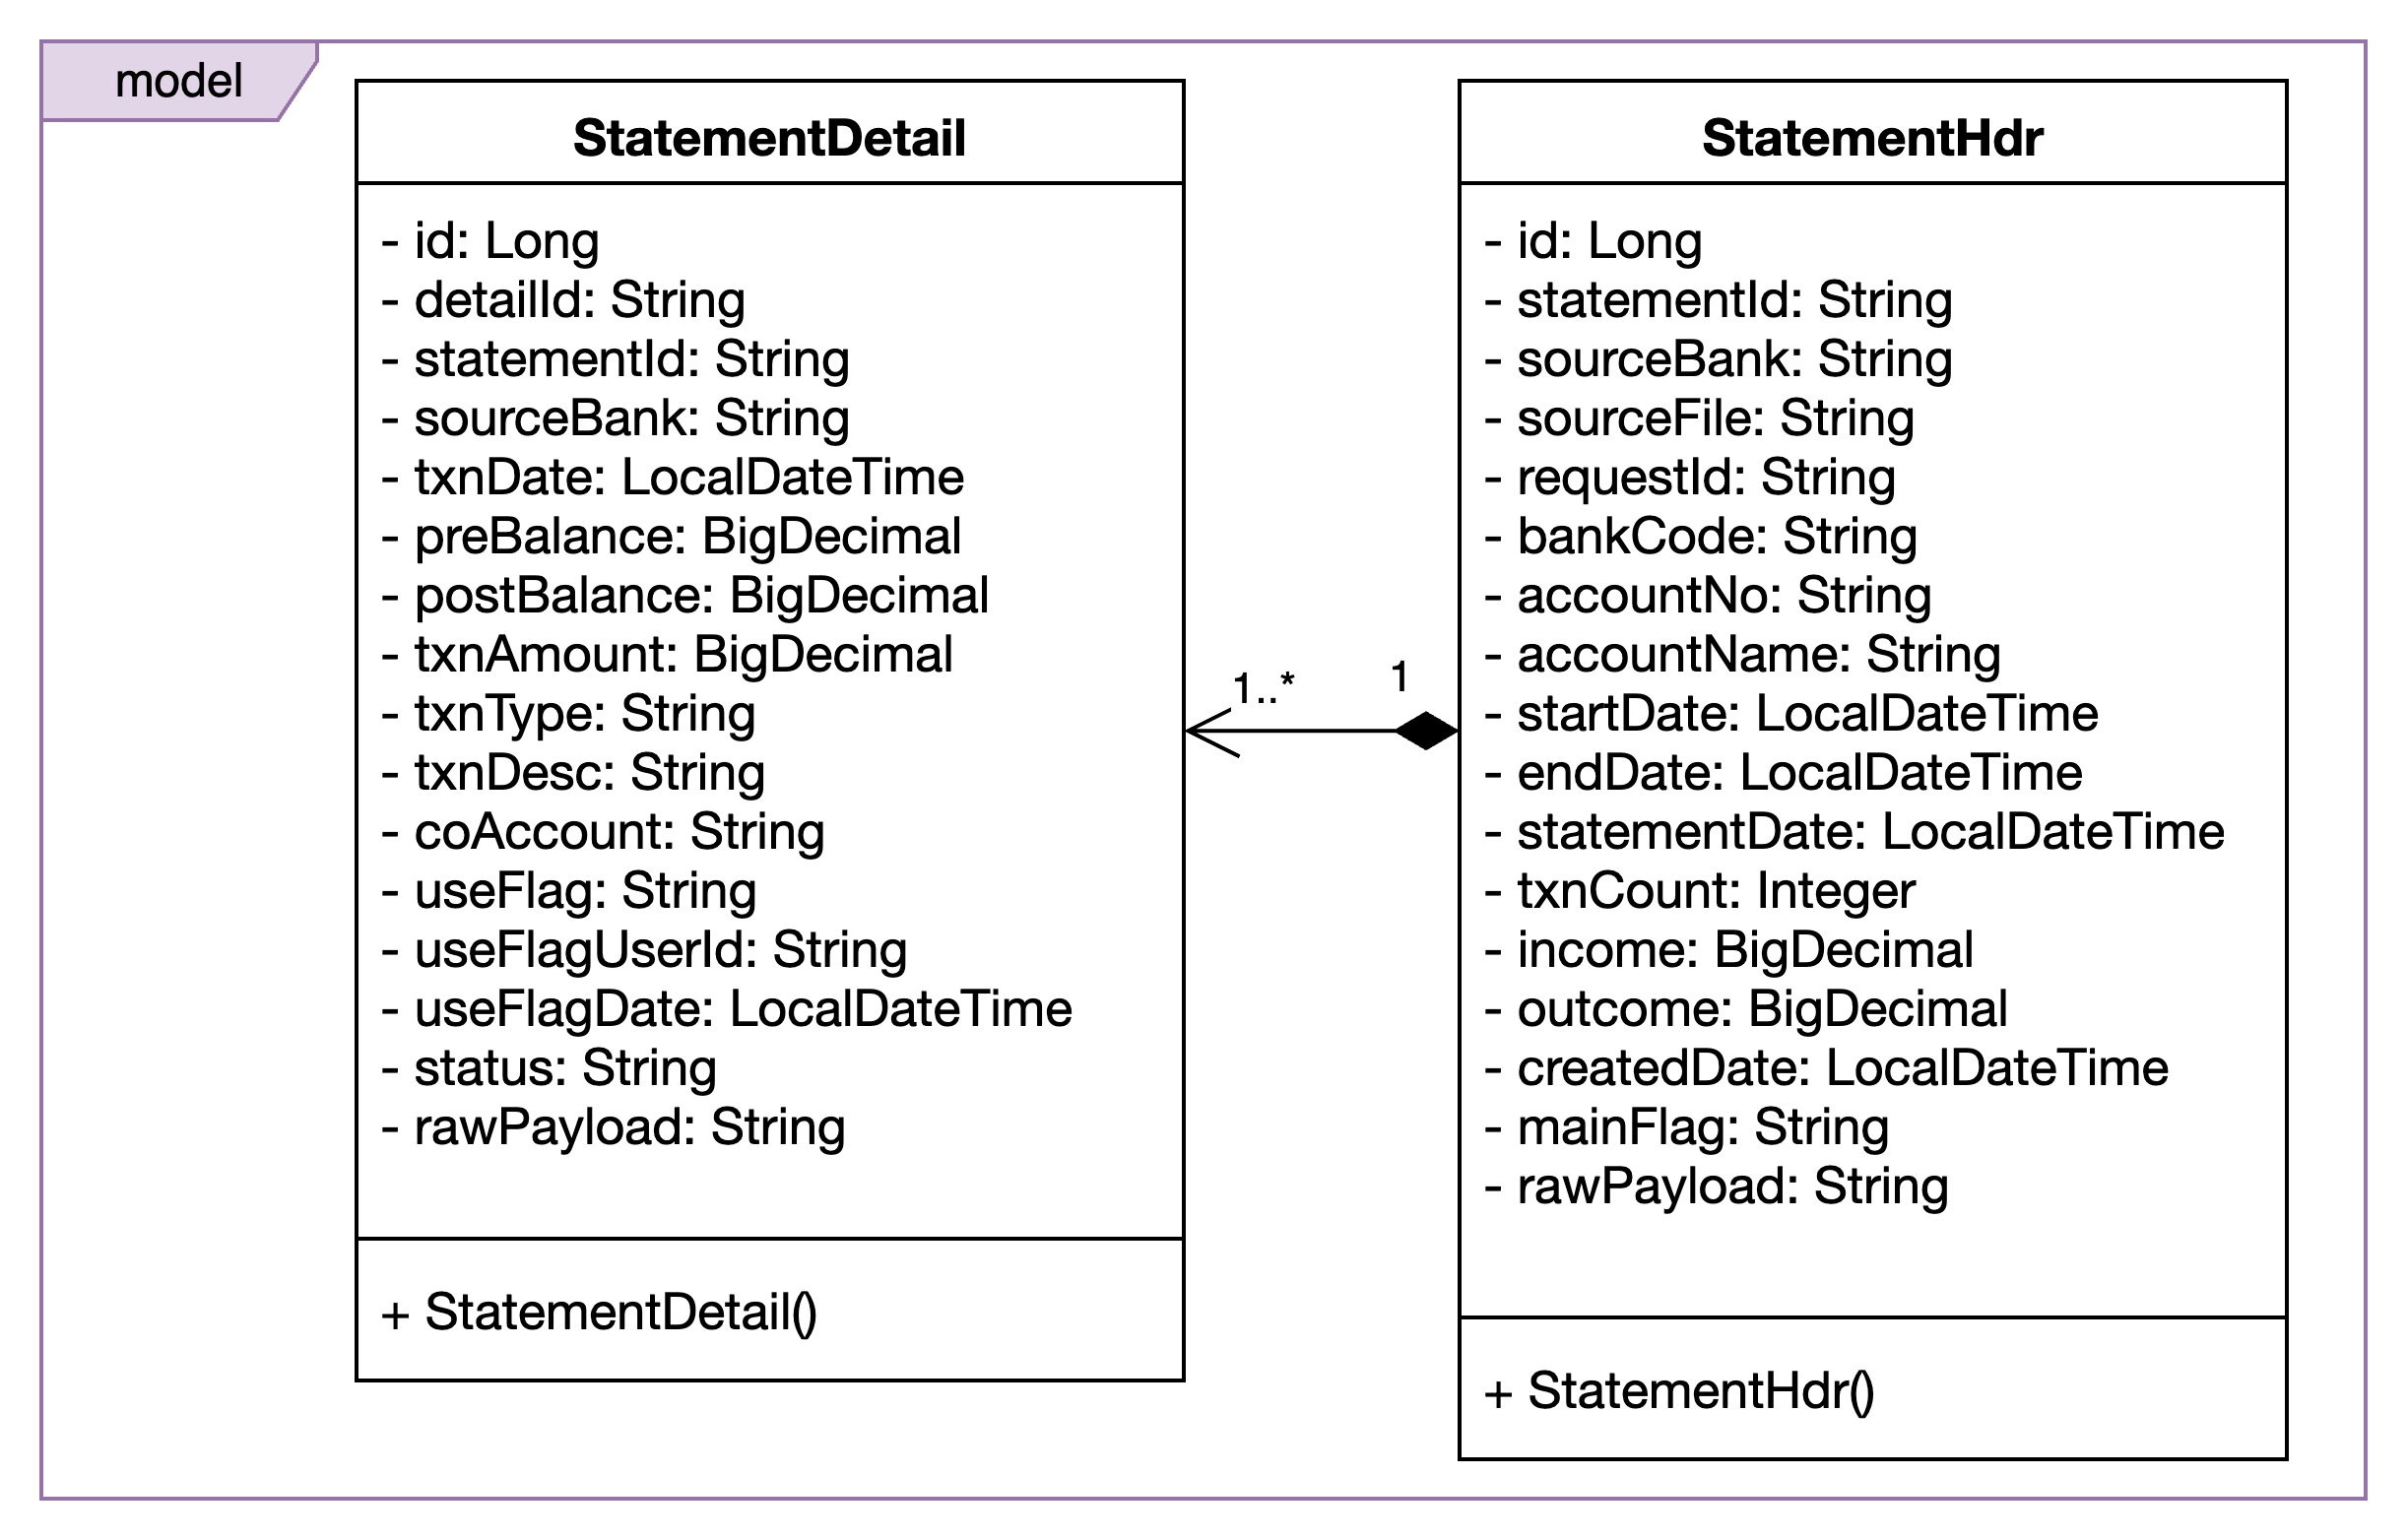
\includegraphics[width=13cm]{images/model.png}
		\caption{MinuPOS системийн банкны Excel хуулгыг боловсруулах модулийн model багцын классын диаграм}
		\label{fig:model}
\end{figure}

\begin{figure}[H]
		\centering
		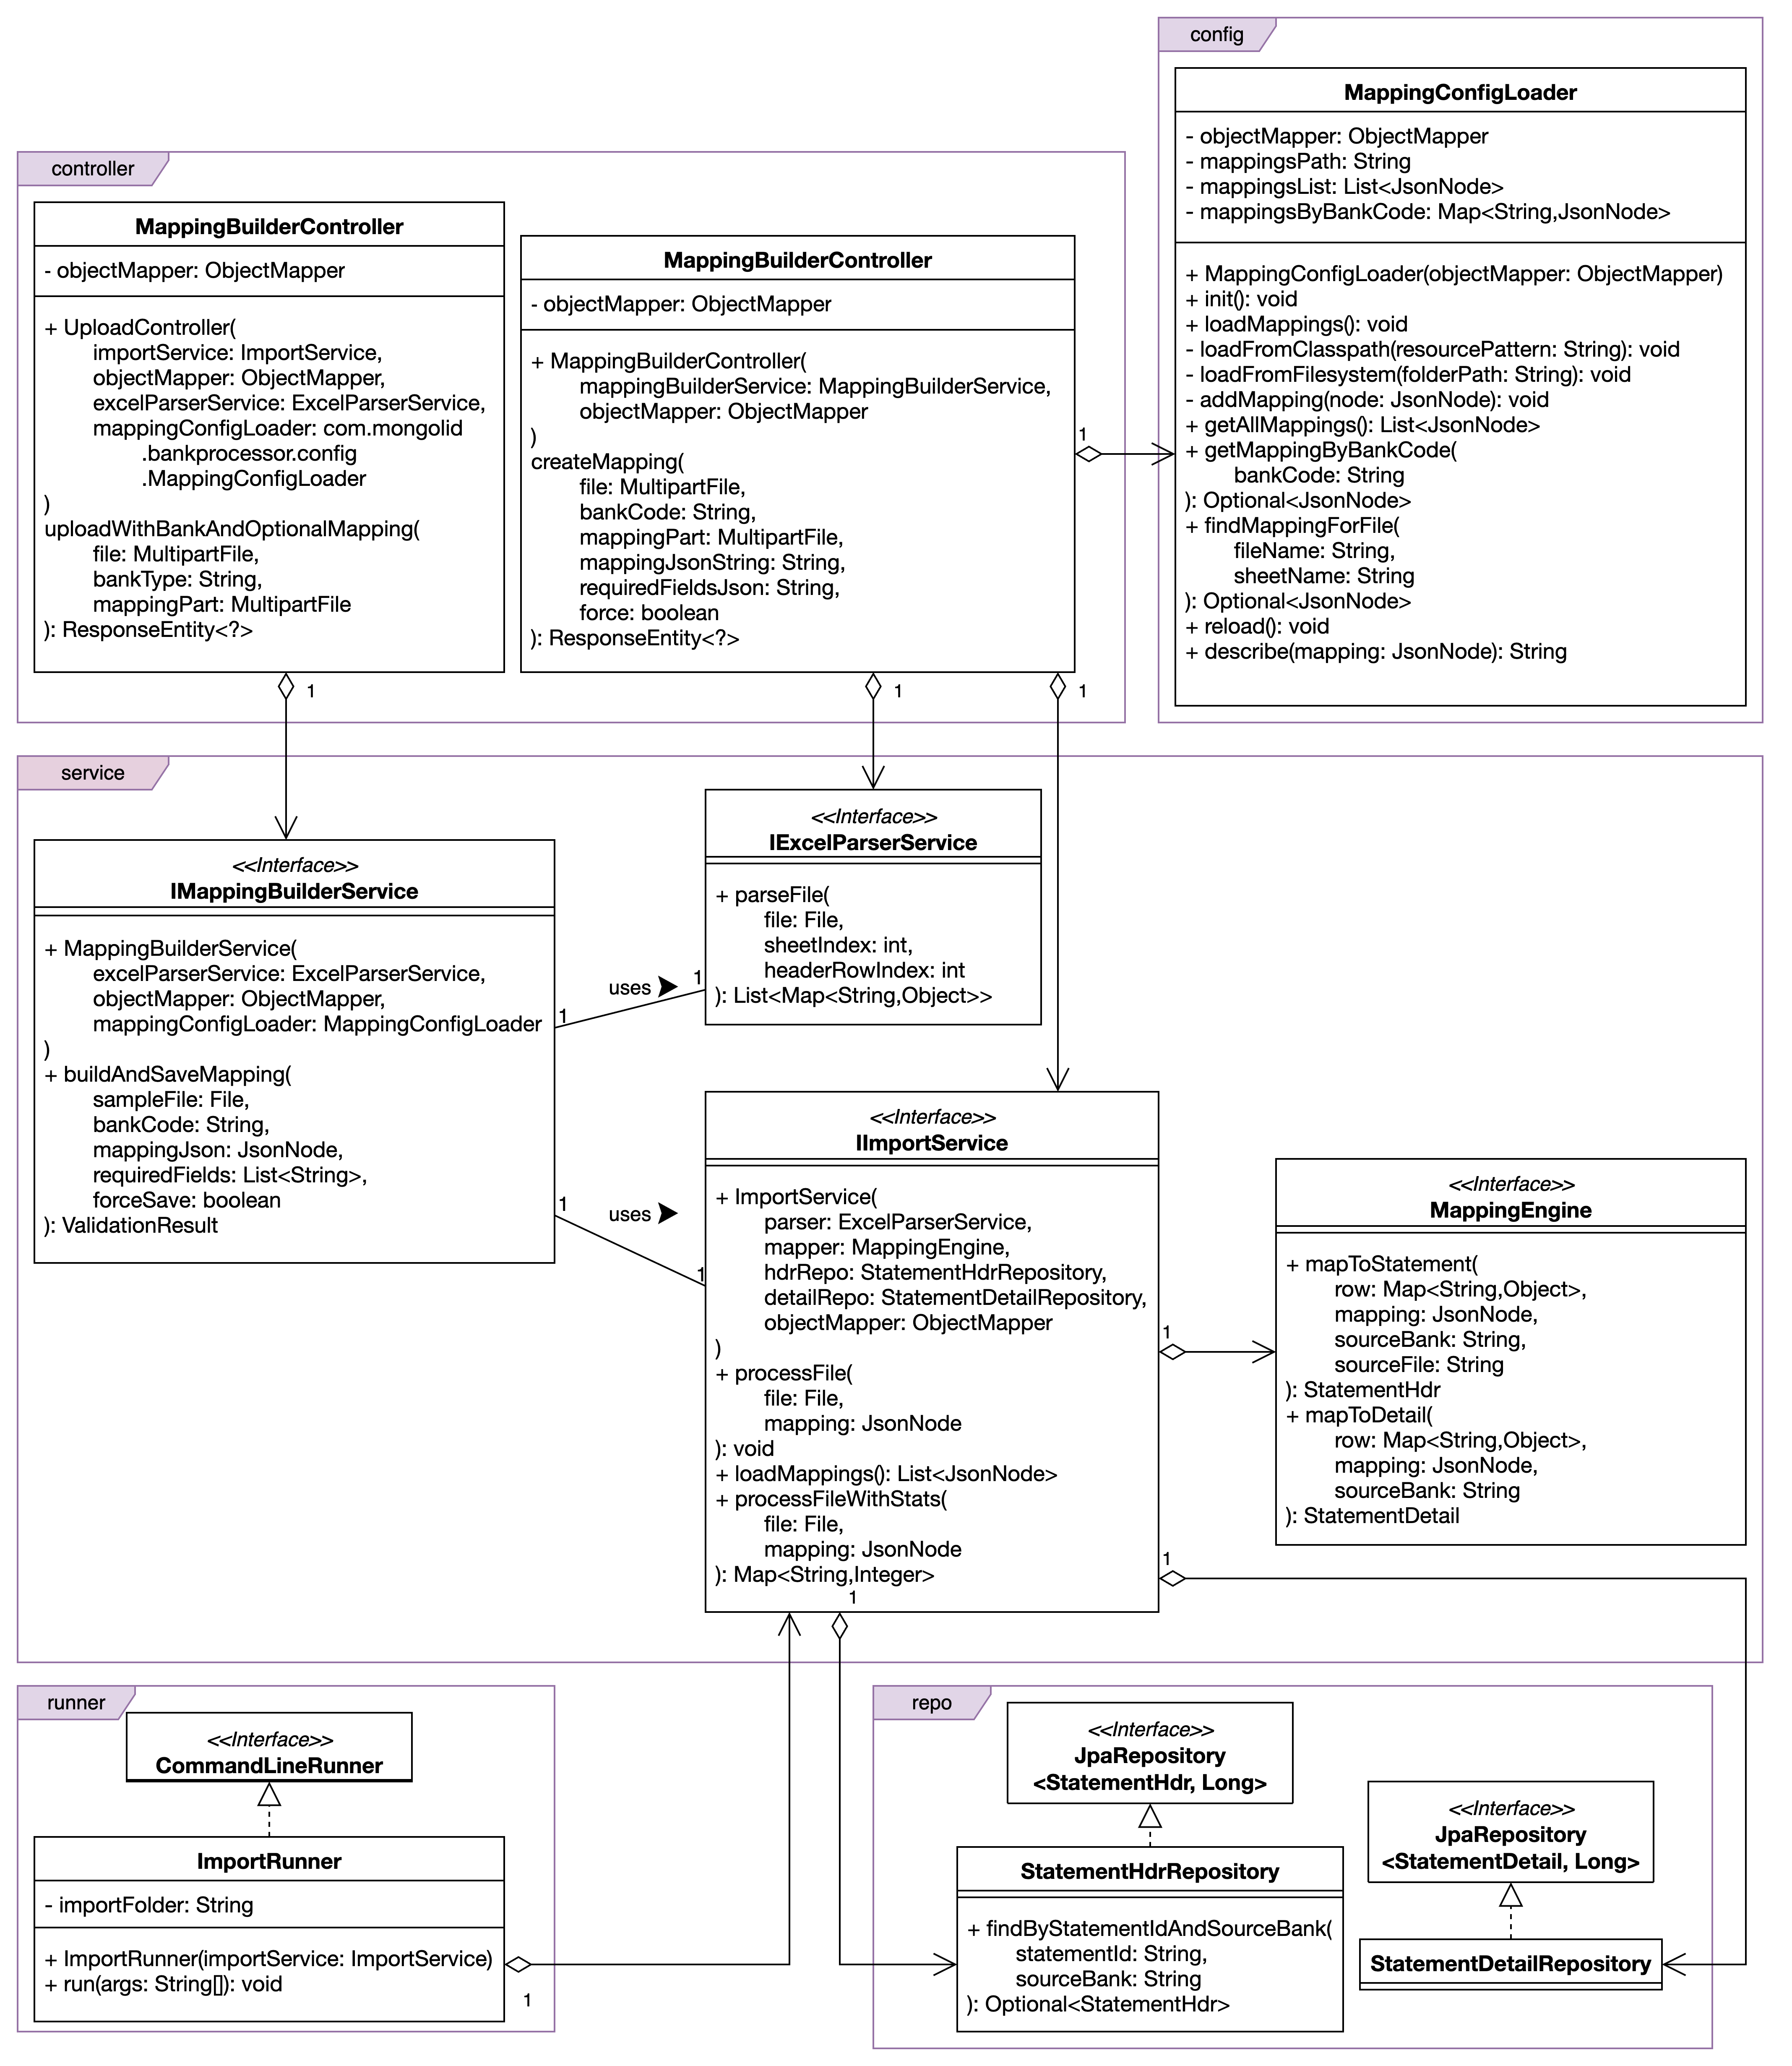
\includegraphics[width=17cm]{images/design.png}
		\caption{MinuPOS системийн банкны Excel хуулгыг боловсруулах модулийн зохиомжийн үеийн классын диаграм}
		\label{fig:design}
\end{figure}

\newpage
\section{MinuPOS системийн банкны Excel хуулгыг боловсруулах модулийн хэрэгжүүлэлт}
